\documentclass[20pt,twocolumn]{article}
\usepackage{geometry}
\geometry{verbose,headsep=3cm,tmargin=2.5cm,bmargin=2.5cm,lmargin=2.0cm,rmargin=2.0cm}
\usepackage{graphicx}
\usepackage{xcolor}
\usepackage[font=small]{caption}
\usepackage{cleveref}
\usepackage{amsmath,amssymb,latexsym}
\usepackage{marvosym}
\usepackage{url}
\usepackage{lipsum}
\usepackage{bm}
\usepackage{float}
\usepackage[english]{babel}
\usepackage{hyperref}
\usepackage{epsf}
\usepackage{float}
\usepackage{mathpazo}
\usepackage{pifont}
\usepackage{wrapfig}
\usepackage{multicol}
\usepackage{enumitem}
\usepackage{xcolor}
\usepackage{framed}
\usepackage[utf8]{inputenc}


\newcommand{\highlight}[1]{%
  \colorbox{orange!50}{$\displaystyle#1$}}

\begin{document}

\twocolumn[{
\begin{@twocolumnfalse}


  \begin{center}

    \vskip-3em

    \hfill
    \textbf{Bruxelles, September 2018}

    \rule{\textwidth}{0.5pt}
    \vskip2ex

    {\Large\textbf{Notes on PCA}}
  
    \vspace{2ex}

      \vspace{1ex}
   
	\texttt{https://camillejr.github.io/science-docs/}
          
  \noindent%
    
\vskip1ex

\rule{\textwidth}{0.5pt}

  \end{center}
  
\vspace{8mm}

\end{@twocolumnfalse}
}]

\vspace{10mm}

\setlength{\parindent}{0cm}

\section*{Acknowledgements}

This document was produced during my PhD at Université libre de Bruxelles.

\section{Introduction}

These are notes on \textbf{Principal Component Analysis} (PCA). They contain everything that I understood or deduced about PCA from absolute zero.

I put a warning here that this document might contain errors, unclear or unreasonable sections. If you would like to help me improve the notes (and my understanding of PCA), feel free to contact me. I will appreciate it very much!

\section{Motivation for data reduction}

There are several questions which stimulated the development of data reduction techniques and reduced-order modelling:

Can we send less information but preserve the resolution of the data (data compression)?

If the data were measurements from an experiment, can we predict what the outcome of another measurement will be?

Can we build a model that will make predictions about a system?

\section{PCA example}

\section{Linear vs. non-linear PCA}

The linear-PCA is adequate for data sets that can be approximated by a linear combination:

\begin{equation}
\text{Data} \approx A_1 \vec{PC1} + A_2 \vec{PC2} + \dots + A_n \vec{PCn}
\end{equation}

where $\vec{PC1}, \vec{PC2}, \dots, \vec{PCn}$ are consecutive principal components (PCs).

The example of a data set that is suited for linear-PCA is presented in Figure \ref{fig:linear_PCA_data}. What is unique about such data set is that it has got a preferred direction in a lower dimension (in this case 1D) along which the data points are aligned. The first PC will be associated with this direction. There will also be a second PC which is perpendicular to the first one, however the weight of this second PC is much lower - there is much less variance of data along this other direction.

The data reduction that we can perform in our heads is that this data set almost aligns with a linear function $f(x) = x$ for $x \in \langle 1; 3 \rangle$.

\begin{figure}[H]
\centering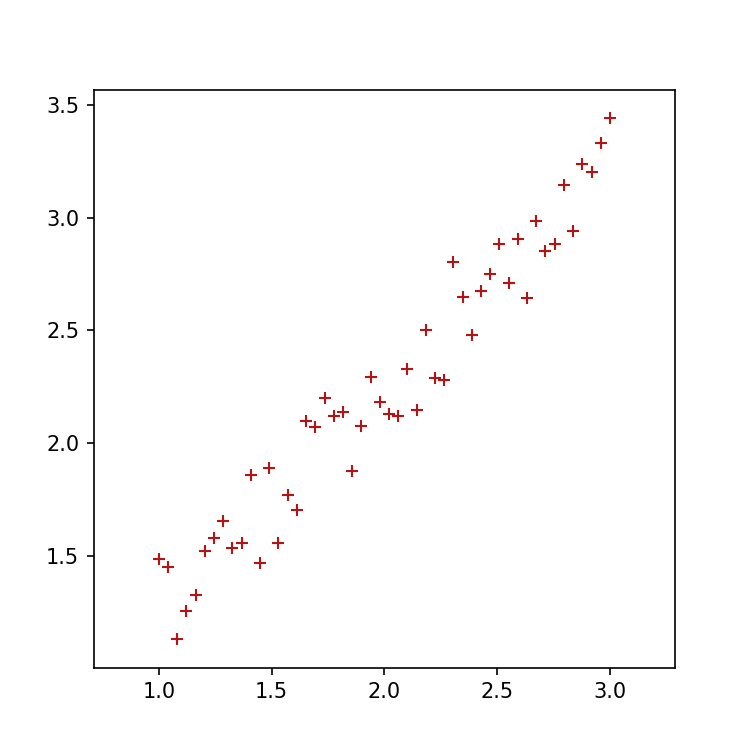
\includegraphics[width=7cm]{../python/PCA-fake-datasets/PCA_linear_scatter_1.png}
\caption{Data set for linear-PCA.}			
\label{fig:linear_PCA_data}
\end{figure}

We may approximate the above data set simply by:

\begin{equation}
\text{Data} \approx A_1 \vec{PC1}
\end{equation}

When we take a look at a data set in Figure \ref{fig:nonlinear_PCA_data}, we can see that the data is spread almost equally along two dimensions. The two PCs of such data set will have almost the same weight (the length of the two eigenvectors will be almost the same). It seems that there is no preferred direction in this data. So, does that mean that it cannot be reduced?

The underlying pattern in this data set is very clearly visible. Intuitively, we can say that the data points are almost aligned with a circle centered at $(2;2)$ with radius $r=1$. If we knew a function $f(x)$ describing that circle, perhaps we might be able to write it in terms of just the first PC and approximate:

\begin{equation}
\text{Data} \approx f(\vec{PC1})
\end{equation}

where $f(\vec{PC1})$ is essentially non-linear.

One idea to find the function $f$ might be to associate the first PC with the radius of the circle (that is find the relation $r(PC1)$) and write:

\begin{equation}
f(x, \vec{PC1})^2 = x^2 + r(\vec{PC1})^2
\end{equation}

This will give us a centered approximation to the original data. 

\begin{figure}[H]
\centering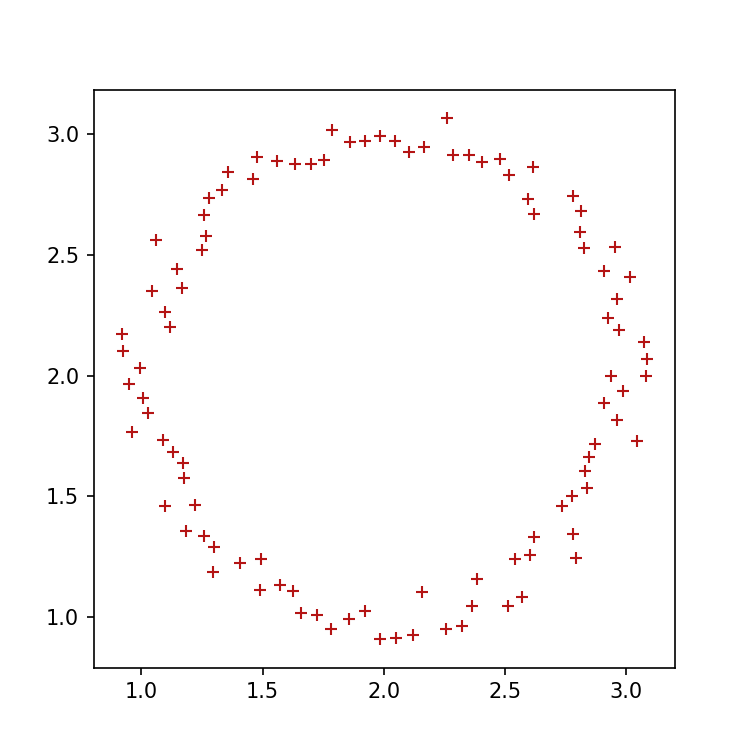
\includegraphics[width=7cm]{../python/PCA-fake-datasets/PCA_nonlinear_scatter_2.png}
\caption{Data set for non-linear-PCA.}			
\label{fig:nonlinear_PCA_data}
\end{figure}

To conclude, the non-linear-PCA is helpful at times when there is no preferred direction in a data set, however there is an underlying non-linear relation that describes the data. The linear-PCA would in such case not give a satisfactory approximation after truncating the number of PCs. 


\section{PC-kriging}



\appendix

\section{APP1} \label{app:A}

\section{APP2} \label{app:B}

\thebibliography{}

\bibitem{Jolliffe} Ian T. Jolliffe \textit{Principal Component Analysis}, Second Edition, 1986
\bibitem{Strang} Gilbert Strang \textit{Introduction to Linear Algebra}, Fifth Edition, 2016

 \label{bib:pope}


\end{document}
